%%%%%%%%%%%%%%%%%%%%%%%%%%%%%%%%%%%%%%%%%%%%%%%%%%%%%%%%%%%%%%%%%%%%%%%%%%%%%%%%%%%%%%%%
%					                       Neural Networks 																	 		 %
%															Academic year 2026/2027                       					 %
%    									  						Lecture 01        								   							 %
%=============== Instrctors: Danilo Comminiello, Simone Scardapane ====================%
%%%%%%%%%%%%%%%%%%%%%%%%%%%%%%%%%%%%%%%%%%%%%%%%%%%%%%%%%%%%%%%%%%%%%%%%%%%%%%%%%%%%%%%%
%
% ---------------------------------------------------
% Template by Danilo Comminiello
% ---------------------------------------------------
\documentclass[xcolor=x11names,compress,10pt,unknownkeysallowed,aspectratio=169]{beamer}
%
% ---------------------------------------------------
% Lecture information
% ---------------------------------------------------
\title{Neural Networks: Course Introduction}
\author[D. Comminiello \& S. Scardapane]{Danilo Comminiello and Simone Scardapane} % Select one
\date{September 25, 2026}
%
% ---------------------------------------------------
% Themes definition
% ---------------------------------------------------
%\makeatletter
%\def\input@path{{../--Template--/}}
%\makeatother
\usetheme{NN26}
%
% ---------------------------------------------------
% Additional commands
% ---------------------------------------------------
%\hyphenation{theo-re-ti-ca-l-ly}
%\graphicspath{{../--Template--/images},{./images/}}

%
% ---------------------------------------------------
% Additional packages
% ---------------------------------------------------
%
% ---------------------------------------------------
% Additional definitions
% ---------------------------------------------------
%
% ---------------------------------------------------
% Begin document
% ---------------------------------------------------
\graphicspath{{assets/}{../../shared/assets/}}
\begin{document}
%
% ---------------------------------------------------
% Background
% ---------------------------------------------------
{\usebackgroundtemplate{
	\vbox to \paperheight{
	\hbox to \paperwidth{\hfil
\includegraphics[keepaspectratio,width=\textwidth]{cover.jpg}\hfil}\vfil}}
	\frame[plain]{\titlepage}
}
%
% ---------------------------------------------------
% Content of the Lecture
% ---------------------------------------------------
%\begin{frame}{Lecture content highlights}
%%
%\begin{beamerboxesrounded}[upper=uppercolLGrayS,lower=lowercolLGrayS,shadow=true]
%{} 
%\begin{itemize}\justifying
	%\vspace{0.7cm}
	%\item We present \alert{goals} and \alert{objectives} of the course.
	%
	%\vspace{0.7cm}
	%\item We give you useful \alert{information} about the course and the exam.
	%
	%\vspace{0.7cm}
	%\item We explain meaning, definition and some history about ``\alert{Neural Networks}''.
	%
%\end{itemize}
%
%\end{beamerboxesrounded}
%\end{frame}
%
% ---------------------------------------------------
% Outline
% ---------------------------------------------------
\begin{frame}{Table of contents}
%\begin{frame}[allowframebreaks]{Table of contents}
\setcounter{tocdepth}{1} % remove subsections from the toc
\tableofcontents[part = 1]
%\tableofcontents[part = 1,sections = {2}]
%\framebreak
%\tableofcontents[part = 1,sections = {3-4}]
\end{frame}
\setcounter{tocdepth}{2} % add subsections from now on
%
% ---------------------------------------------------
% Section 1
% ---------------------------------------------------
\part[Lecture 1]{1}
\section[\scshape\bfseries About The Course]{\scshape\bfseries About The Course}
%
% ---------------------------------------------------
% New frame
% ---------------------------------------------------
\subsection{Teachers}
\begin{frame}{Your teachers}
\begin{columns}
	\begin{column}{0.6\textwidth}
	%
	\begin{figure}
		\centering
		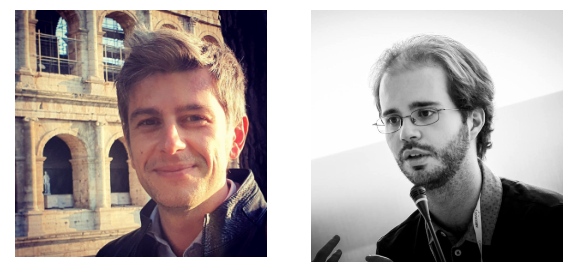
\includegraphics[width=0.77\columnwidth, keepaspectratio]{Teachers2023.png}
		%\caption{}
	\end{figure}
	\end{column}
	%
	\begin{column}{0.45\textwidth}
		\begin{itemize}\justifying
			\item \alert{Danilo Comminiello}
			
			\myhref{https://danilocomminiello.site.uniroma1.it/}{danilocomminiello.site.uniroma1.it}
			
			danilo.comminiello@uniroma1.it
			
			\vspace{0.5cm}
			\item \alert{Simone Scardapane}
			
			\myhref{https://www.sscardapane.it/}{www.sscardapane.it}
			
			simone.scardapane@uniroma1.it
			
			%\vspace{0.2cm}
			%\alert{\rule{0.9\columnwidth}{0.02cm}}
			%\vspace{0.2cm}
			%
			%\alert{Offices:} DIET, 1\textsuperscript{st} floor
			%
			%\alert{Laboratory:} \myhref{www.ispamm.it}{ISPAMM Lab}, DIET% Dept., 1\textsuperscript{st} floor
			%
			%\alert{Office hours:} by appointment
		\end{itemize}
	\end{column}
\end{columns}
\end{frame}
%
% ---------------------------------------------------
% New frame
% ---------------------------------------------------
\subsection{General Information}
\begin{frame}{General information}
\begin{itemize}\justifying
	\item \alert{Credits:} 6 CFU
	
	\vspace{0.2cm}
	\item \alert{Course language:} English
	
	\vspace{0.2cm}
	\item \alert{Offered programs:} Master's Degrees in Artificial Intelligence and Robotics, Engineering in Computer Science, optional for any course of study
	
	\vspace{0.2cm}
	\item \alert{Course webpage:} \myhref{https://sites.google.com/uniroma1.it/neuralnetworks2026/}{https://sites.google.com/uniroma1.it/neuralnetworks2026/}
	
	\vspace{0.2cm}
	\item \alert{Classroom page:} Download slides, notebooks, and additional material. Also used for news and important communications. Access code: \textbf{sy3uqdop
}. Please register \myhref{https://classroom.google.com/c/MTYyNjk5MDA2NzU3?cjc=7uynqjmd}{here}.
	
	\vspace{0.2cm}
	\item \alert{Offices:} DIET Dept. (SPV), RM032, 1\textsuperscript{st} floor

	\vspace{0.2cm}
	\item \alert{Office hours:} by appointment
	
	\vspace{0.2cm}
	\item \alert{Laboratory:} \myhref{www.ispamm.it}{ISPAMM Lab}, DIET Dept.
\end{itemize}
\end{frame}
%
% ---------------------------------------------------
% New frame
% ---------------------------------------------------
\begin{frame}{ISPAMM Research Lab}
%\vspace{0.5cm}
\begin{figure}[t]
\centering
	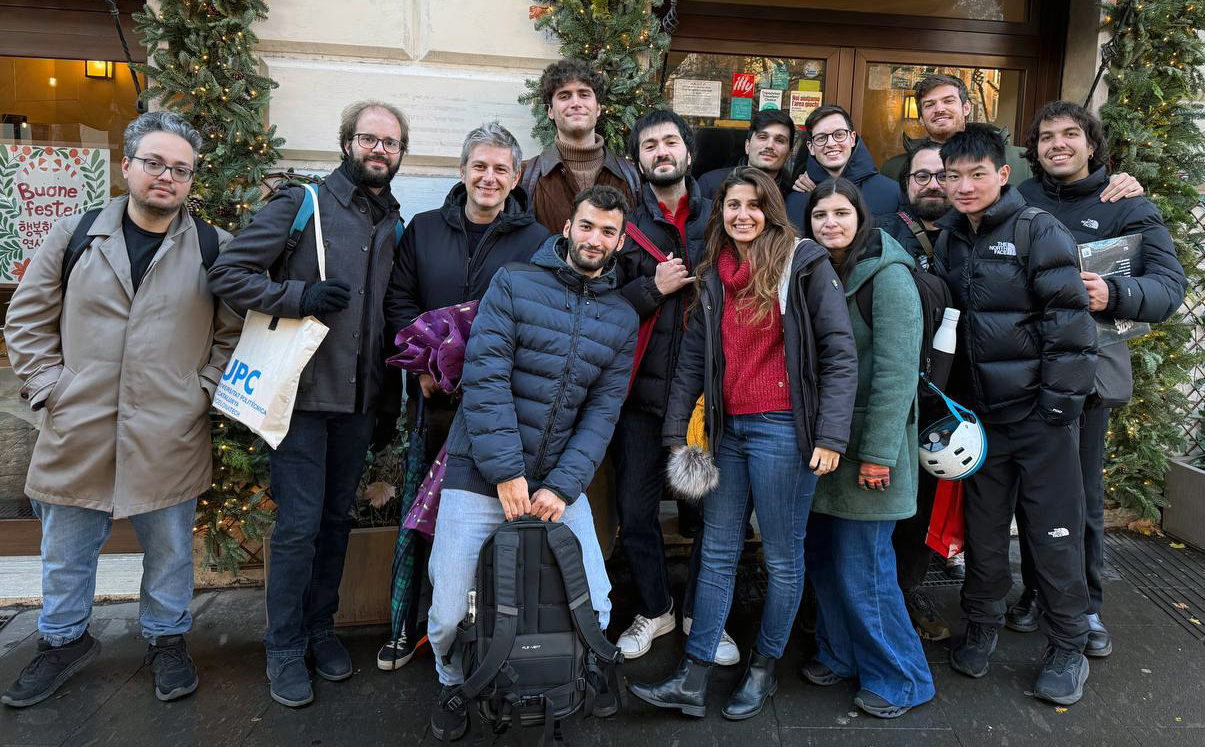
\includegraphics[width=0.75\textwidth,keepaspectratio]{ISPAMMlab_2024-12-20.jpg}
	%\vspace{0.1cm}
	\caption{The \alert{\textbf{Intelligent Signal Processing and MultiMedia (ISPAMM)}} research team (Website: \myhref{www.ispamm.it}{www.ispamm.it}).
	}
\end{figure}
\vfill
\end{frame}
%
% ---------------------------------------------------
% New frame
% ---------------------------------------------------
\subsection{Course Description}
\begin{frame}{Course description}
The course is intended as a \alert{broad overview to neural networks}, as used today in a number of applicative fields.

\vspace{0.6cm}
It provides both \alert{theoretical and practical understanding} of how neural networks are \linebreak designed and implemented.

% \vspace{0.6cm}
% We will review the general paradigm of building \alert{differentiable models}.

\vspace{0.6cm}
We explore how to address \textit{machine learning} and \textit{deep learning} tasks with \alert{neural networks}.

\vspace{0.6cm}
We introduce \alert{essential components} to deal with images (\textit{convolutive layers}), sequences (\textit{recurrent layers}), and sets (\textit{transformer layers}).

\vspace{0.6cm}
We finally focus on a selection of \alert{advanced and emerging topics}, including \textit{multimodal neural networks} and \textit{explainability}, among others.
\end{frame}
%
% ---------------------------------------------------
% New frame
% ---------------------------------------------------
\subsection{Expected Results}
\begin{frame}{Expected results}
At the end of the course, a student is expected to have:

\vspace{0.2cm}
\begin{itemize}\justifying
	\item a broad understanding of \alert{how neural networks work} in practice, 
	
	\vspace{0.2cm}
	\item the capability of \alert{implementing new components} from scratch, 
	
	\vspace{0.2cm}
	\item the capability of \alert{re-using existing models}, 
	
	\vspace{0.2cm}
	\item the capability of \alert{designing new architectures} for problems beyond the overview of the course,
	
	\vspace{0.2cm}
	\item the ability to \alert{autonomously study new topics} on the research frontier, and navigate the current scientific literature and software panorama.
\end{itemize}
\end{frame}
%
% ---------------------------------------------------
% New frame
% ---------------------------------------------------
\begin{frame}{What we expect you to do}
\begin{itemize}\justifying
    \item Be \alert{curious} and \alert{passionate} about AI and Neural Networks.

    \vspace{0.7cm}
	\item Ask yourself what your main \alert{interests in Neural Networks} are.

	\vspace{0.7cm}
	\item Consider the practical part of this course as an opportunity for you to \alert{understand your attitudes}.
		
	\vspace{0.7cm}
	\item \alert{Attend classes}, as it is the first step to become an \alert{AI master}!
\end{itemize}
\end{frame}
%
% ---------------------------------------------------
% New frame
% ---------------------------------------------------
\begin{frame}{Prerequisites and background}
This course requires \alert{basic knowledge} of:

\vspace{0.2cm}
\begin{itemize}\justifying
	\item machine learning fundamentals

	\vspace{0.2cm}
	\item linear algebra
	
	\vspace{0.2cm}
	\item probability theory and stochastic processes

	\vspace{0.2cm}
	\item optimization
	
	\vspace{0.2cm}
	\item Python
\end{itemize}

\vspace{0.4cm}	
Anyway, sufficient \alert{recalls} will be given and \alert{additional material} can be provided, even on request, to fill some gaps.
\end{frame}
%
% ---------------------------------------------------
% New frame
% ---------------------------------------------------
\subsection{Syllabus}
\begin{frame}[allowframebreaks]{Syllabus}
%
\begin{itemize}\justifying
	\item \alert{\textbf{Introduction and Background}}
	\begin{itemize}\justifying
		\small{
		\vspace{0.1cm}
		\item[$-$] Introduction to neural networks
		\vspace{0.1cm}
		\item[$-$] Background recalls on linear algebra, probability and optimization, computation
	}\normalsize
	\end{itemize}
	\vspace{0.3cm}
	\item \alert{\textbf{Neural Networks Fundamentals}}
	\begin{itemize}\justifying
	\small{
		\vspace{0.1cm}
		\item[$-$] Linear regression, training and automatic differentiation
    	\vspace{0.1cm}
		\item[$-$] Multi-layer perceptrons
	}\normalsize
	\end{itemize}
	\vspace{0.3cm}
	\item \alert{\textbf{Core Neural Network Models}}
	\begin{itemize}\justifying
	\small{
		\vspace{0.1cm}
		\item[$-$] Convolutional neural networks and modern architectures
            \vspace{0.1cm}
		\item[$-$] Recurrent neural networks and modern architectures
            \vspace{0.1cm}
		\item[$-$] Transformers and attention-based architectures
			\vspace{0.1cm}
		\item[$-$] Graph neural networks
	}\normalsize
	\end{itemize}
%        \vspace{0.3cm}

\framebreak
	\item \alert{\textbf{Efficient Neural Networks}}
	\begin{itemize}\justifying
	\small{
		\vspace{0.1cm}
		\item[$-$] Quantization and pruning 
            \item[$-$] Dynamic sparsity
						\vspace{0.1cm}
            \item[$-$] Hypercomplex neural networks
	}\normalsize
	\end{itemize}
	\vspace{0.3cm}
	\item \alert{\textbf{Multimodal Neural Networks}}
	\begin{itemize}\justifying
	\small{
		\vspace{0.1cm}
		\item[$-$] Multimodal representation learning
		\vspace{0.1cm}
		\item[$-$] Joint embedding predictive architectures
		\vspace{0.1cm}
		\item[$-$] Large-scale multimodal networks
	}\normalsize
	\end{itemize}
	\vspace{0.3cm}
	%\item \alert{\textbf{Generative Models}}
	%\begin{itemize}\justifying
	%\small{
		%\vspace{0.1cm}
		%\item[$-$] Generative modeling approach
   	    %\vspace{0.1cm}
		%\item[$-$] Diffusion models: tasks and applications
	%}\normalsize
	%\end{itemize}
	%\vspace{0.3cm}
	\item \alert{\textbf{Explainability and Interpretability}}
	\begin{itemize}\justifying
	\small{
		\vspace{0.1cm}
		\item[$-$] Explainability techniques and case studies
%            \item[$-$] Case studies
	}\normalsize
	\end{itemize}
\end{itemize}
\end{frame}
%
% ---------------------------------------------------
% New frame
% ---------------------------------------------------
\begin{frame}{Course material}
\alert{\textbf{General information:}}
%
\begin{itemize}\justifying
		\item {\small{On the \myhref{https://sites.google.com/uniroma1.it/neuralnetworks2026/}{NN course page} you can find all the course information, including program and exam dates.}}
\end{itemize}

\vspace{0.4cm}
\alert{\textbf{Main material:}}
	%
\begin{itemize}\justifying
	\item {\small{Lecture slides, papers, notebooks, supplementary material, and news will be provided on the \myhref{hhttps://classroom.google.com/c/MTYyNjk5MDA2NzU3?cjc=7uynqjmd}{Classroom page} (access code: 7uynqjmd).}}
\end{itemize}

%\vspace{0.4cm}
%\alert{\textbf{GitHub:}}
%%
%\begin{itemize}\justifying
		%\item {\small{XX}}
%\end{itemize}
%
\vspace{0.4cm}
%
\alert{\textbf{Main textbooks (available online):}}
%
\begin{itemize}\justifying
            \item {\small{Simone Scardapane, ``\myhref{https://www.sscardapane.it/alice-book/}{Alice’s Adventures in a Differentiable Wonderland}", 2024.}}
		\item {\small{Simon J. D. Prince, ``\myhref{https://udlbook.github.io/udlbook/}{Understanding Deep Learning}'', MIT Press, 2023.}}
		\item {\small{Aston Zhang, Zachary C. Lipton, Mu Li, and Alexander J. Smola, ``\myhref{https://d2l.ai/}{Dive Into Deep Learning}'', 2023.}}
\end{itemize}
\end{frame}
%
% ---------------------------------------------------
% New frame
% ---------------------------------------------------
\subsection{Class Schedule}
\begin{frame}{Class schedule}
The course starts on \alert{September 25, 2026} and will end on \alert{December 18, 2026}, with the following schedule:
%
\vspace{0.2cm}
\begin{itemize}\justifying
    \item Tuesday, 13:30--16:00, Classroom A3, Via Ariosto, 25
    \item Friday, 12:00--13:30, Classroom A5, Via Ariosto, 25
\end{itemize}

\vspace{0.5cm}
The course is held in \alert{in-presence modality} only.
\end{frame}
%
% ---------------------------------------------------
% New frame
% ---------------------------------------------------
\subsection{Exam Assessment}
\begin{frame}{Exam assessment and grade evaluation}
\begin{itemize}\justifying
		
	\vspace{0.3cm}
	\item \alert{\textbf{Default option}}
	\small{
		\begin{itemize}\justifying
			\vspace{0.1cm}
			\item[$-$] \alert{Oral} examination on the course program (usually 2 topics).
			
		\end{itemize}
	}\normalsize

	\vspace{0.6cm}
	\item \alert{\textbf{Research option}}
	\small{
		\begin{itemize}\justifying
			\vspace{0.1cm}
			\item[$-$] \alert{Research projects} on emerging and advanced topics (proposed by professors only).

			\vspace{0.1cm}
			\item[$-$] It could be useful to run for the \alert{lode} or to prepare for a possible follow-up \alert{thesis}.
		\end{itemize}
	}\normalsize	
\end{itemize}

\end{frame}
%
% ---------------------------------------------------
% New frame
% ---------------------------------------------------
\begin{frame}{Exam schedule}
\begin{itemize}\justifying
	\item \alert{\textbf{I Session:}} January TBD, 2027
	
	\vspace{0.3cm}
	\item \alert{\textbf{II Session:}} February TBD, 2027
	
	\vspace{0.3cm}
	\item \alert{\textbf{I Extraordinary Session:}} March TBD, 2027

        \vspace{0.3cm}
	\item \alert{\textbf{III Session:}} June TBD, 2027
		
	\vspace{0.3cm}
	\item \alert{\textbf{IV Session:}} July TBD, 2027
	
	\vspace{0.3cm}
	\item \alert{\textbf{V Session:}} September TBD, 2027
	
	\vspace{0.3cm}
	\item \alert{\textbf{II Extraordinary Session:}} October TBD, 2027
\end{itemize}
\end{frame}
%
% ---------------------------------------------------
% Section 2
% ---------------------------------------------------
\section[\scshape\bfseries Sec 2]{\scshape\bfseries What are neural networks?}
%
% ---------------------------------------------------
% New frame
% ---------------------------------------------------
\subsection{Neural Networks Daily}
\begin{frame}{Neural networks are everywhere}
		
	\begin{figure}
		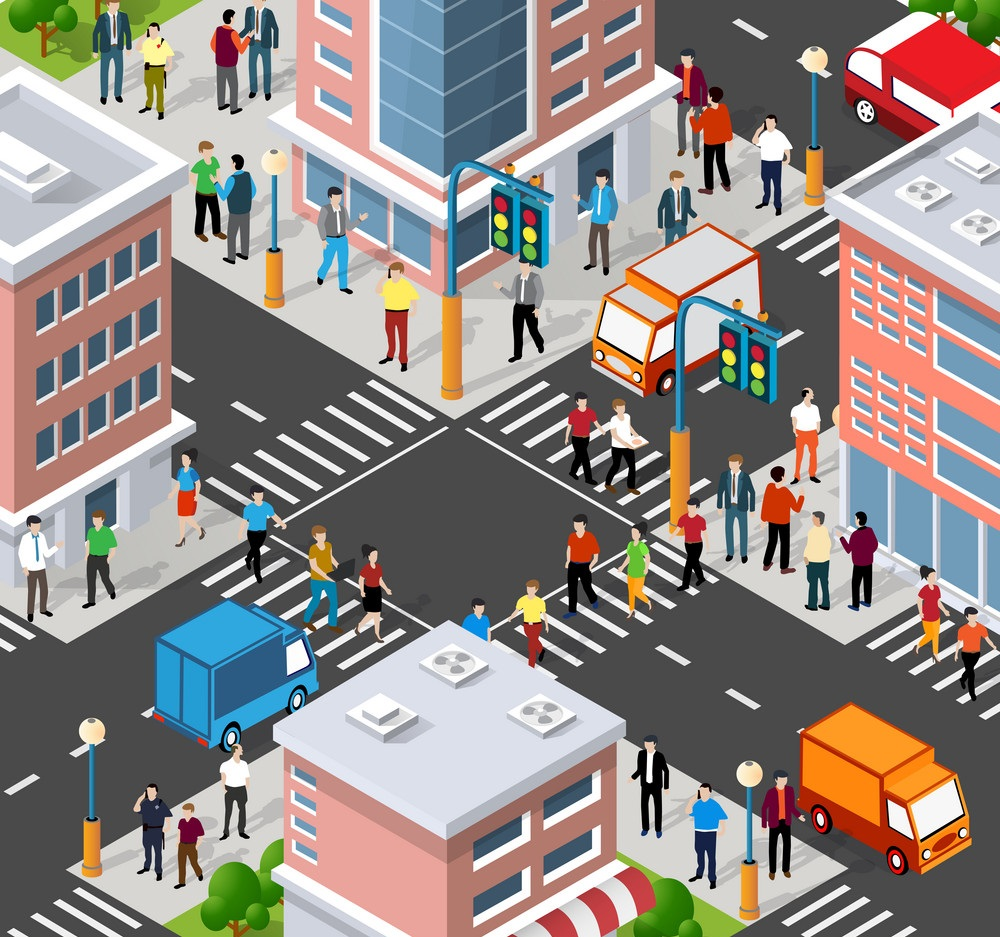
\includegraphics[height=0.85\textheight]{isometric-people-walking-on-street-vector-29295876}
	\end{figure}
		
\end{frame}
%
% ---------------------------------------------------
% New frame
% ---------------------------------------------------
\begin{frame}{Neural networks are everywhere}
		
	\begin{figure}
		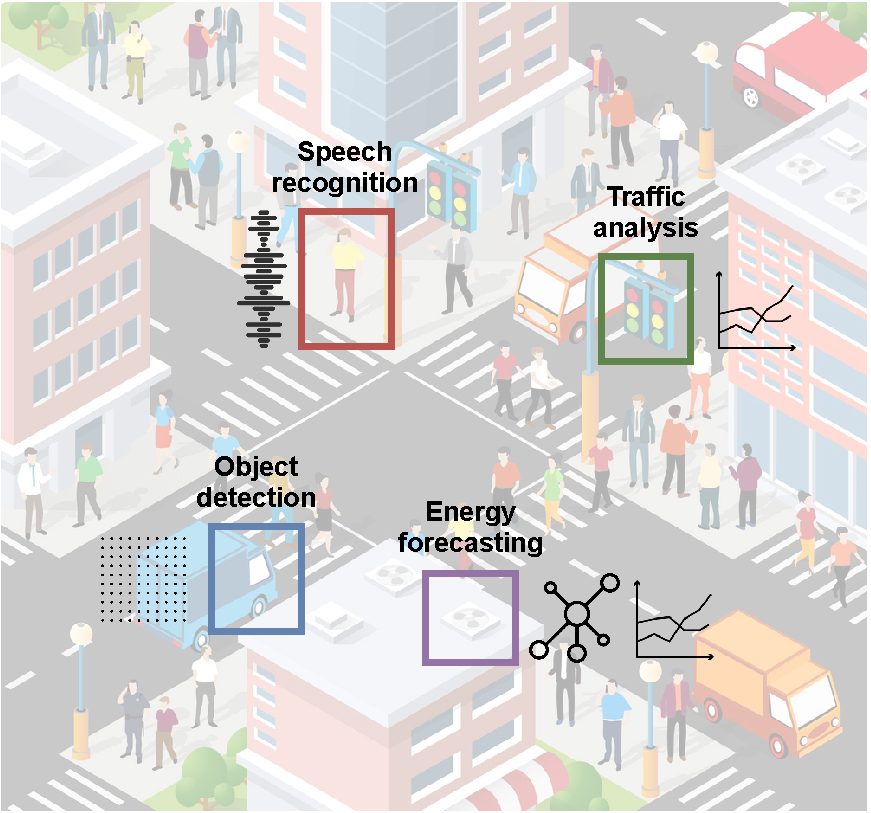
\includegraphics[height=0.85\textheight]{NeuralNetworksArePervasive}
	\end{figure}
	
\end{frame}
%
% ---------------------------------------------------
% New frame
% ---------------------------------------------------
\begin{frame}{Neural networks daily}
Neural networks \alert{power many AI applications} we use every day, often without realizing it.

\vspace{0.5cm}
Examples of AI systems relying on neural networks, among others:
\vspace{0.1cm}

\begin{itemize}
    \item \alert{Voice Assistants:} Siri, Alexa, etc., use speech recognition systems.
    
    \vspace{0.3cm}
    \item \alert{Image Tagging:} Social media platforms automatically tag faces in photos.

    \vspace{0.3cm}
    \item \alert{Recommendation Systems:} Streaming services suggest movies and music.

    \vspace{0.3cm}
    \item \alert{Autonomous Driving:} Modern cars use neural networks for object detection and navigation.
\end{itemize}
  
% Possible figure: Insert a collage or a set of icons representing these real-world applications.
\end{frame}
%
% ---------------------------------------------------
% New frame
% ---------------------------------------------------
\subsection{Definition of Neural Networks}
\begin{frame}{What is a neural network?}
Neural networks are \alert{\textbf{composable}}, \alert{\textbf{differentiable}}, and \alert{\textbf{parameterized functions}} that can be optimized end-to-end using gradient-based methods.

\vspace{0.4cm}
\begin{figure}[h]
  \centering
  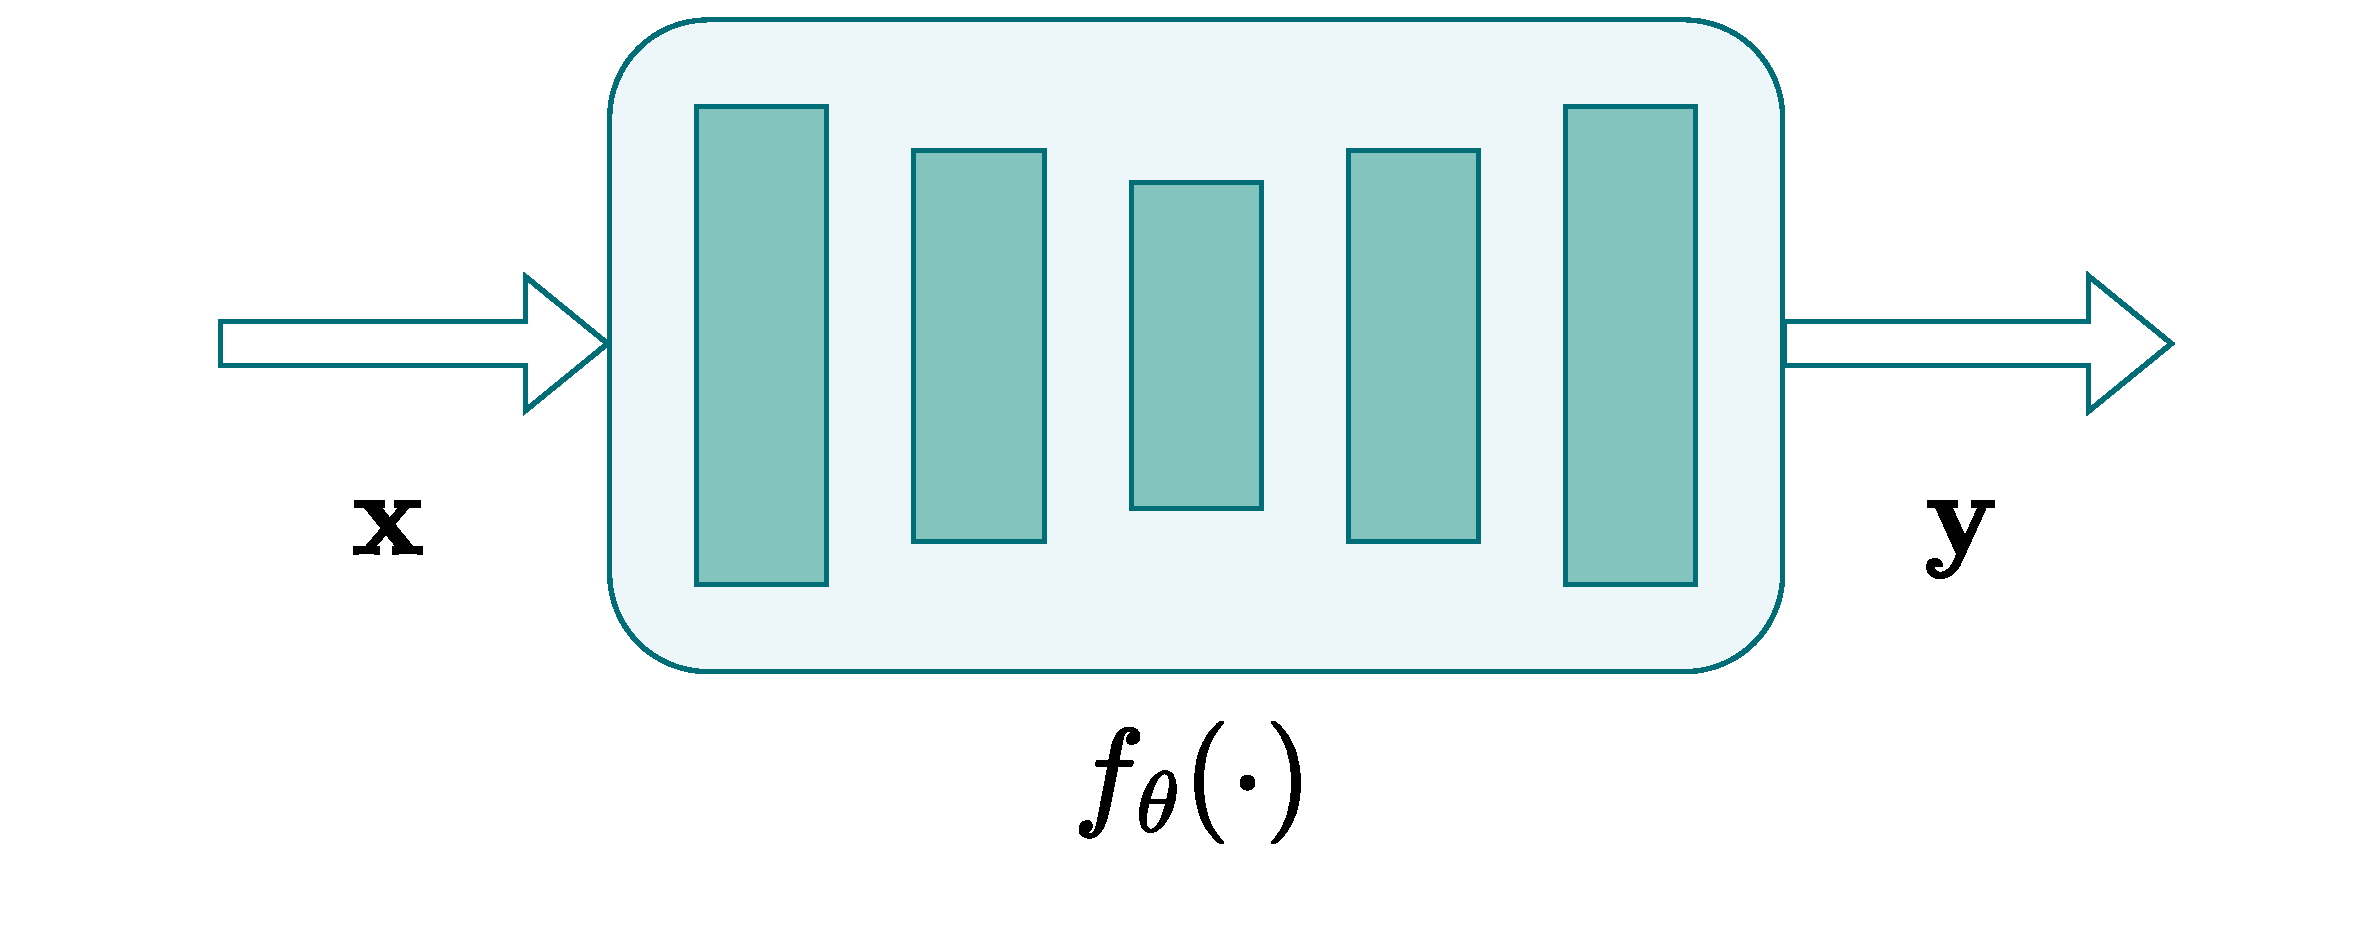
\includegraphics[width=0.65\linewidth]{NNscheme.pdf}
  %\caption{A simple neural network architecture.}
\end{figure}

%\vspace{0.1cm}
They consist of \alert{interconnected layers} (\textit{processing blocks}) that extract hierarchical features from complex, high-dimensional data.

\vspace{0.2cm}
This design enables them to \alert{learn intricate patterns} and representations from raw inputs.

\end{frame}
%
% ---------------------------------------------------
% New frame
% ---------------------------------------------------
\begin{frame}{Neural networks as processing blocks of complex data}
A neural network functions as a \alert{processing block} that converts complex inputs into meaningful outputs.

\vspace{0.6cm}
\alert{Data flow:}
\vspace{0.1cm}
\begin{enumerate}
    \item \textit{Input:} Raw data (e.g., images, text, audio).
    
    \vspace{0.3cm}
    \item \textit{Hidden Processing:} Sequential layers extract and transform features.

    \vspace{0.3cm}
    \item \textit{Output:} Final predictions (e.g., class labels, regression values).
\end{enumerate}

\vspace{0.6cm}
This modular scheme simplifies handling and \alert{understanding complex, high-dimensional data}.
  
% Possible figure: Add a figure depicting the flow of data through a neural network. Or a figure of a block processing unstructured complex data.
\end{frame}
%
% ---------------------------------------------------
% New frame
% ---------------------------------------------------
\begin{frame}{Modular structure of neural networks}
Neural networks are built from simple computational blocks called \alert{neurons}.

\vspace{0.6cm}
These neurons are organized into layers:
\vspace{0.1cm}
\begin{itemize}
    \item \alert{Input Layer:} Receives raw data.
    
    \vspace{0.3cm}
    \item \alert{Hidden Layers:} Process and extract features.

    \vspace{0.3cm}
    \item \alert{Output Layer:} Produces the final prediction or classification.
\end{itemize}

\vspace{0.6cm}
Each layer applies a \alert{simple transformation}; their composition yields a powerful model.

  
% Possible figure: Insert a block diagram illustrating the layer-wise structure.
\end{frame}
%
% ---------------------------------------------------
% New frame
% ---------------------------------------------------
\begin{frame}{Key components of a neural network}
\alert{Neurons:} The basic units that perform simple computations.

\vspace{0.8cm}
\alert{Weights \& biases:} Parameters that scale and shift the input signals.

\vspace{0.8cm}
\alert{Activation functions:} Introduce non-linearity to enable complex decision boundaries.

\vspace{0.8cm}
\alert{Layers:} Groups of neurons that work together to process data.
  
% Possible figure: Consider adding a diagram that labels these components within a typical layer.
\end{frame}
%
% ---------------------------------------------------
% New frame
% ---------------------------------------------------
\begin{frame}{Learnable parameters}
All inputs and outputs are represented as \alert{tensors}---large, $n$-dimensional arrays of numbers.

\vspace{0.6cm}
Neural networks consist of multiple blocks (\alert{layers}), each performing a simple operation on these tensors.

\vspace{0.6cm}
Each layer uses \alert{parameters} (e.g., in a matrix multiplication) that adjust the input data. These parameters are \alert{learned} during training.

\vspace{0.6cm}
The entire network is \alert{optimized} end-to-end via numerical methods, improving its \linebreak performance on a given \alert{dataset}.
\end{frame}
%
% ---------------------------------------------------
% New frame
% ---------------------------------------------------
\begin{frame}{Differentiability and end-to-end optimization}
The differentiable nature of neural networks allows the use of \alert{gradient-based optimization techniques}.

\vspace{0.8cm}
\alert{End-to-end training:} All parameters are adjusted simultaneously to minimize a \textit{loss function} over a training dataset.

\vspace{0.8cm}
This smooth, numerical optimization is key to the network’s ability to \alert{learn from data}.
  
% Possible figure: Insert a simple flowchart illustrating the training loop (forward pass, loss computation, backpropagation, parameter update).
\end{frame}
%
% ---------------------------------------------------
% New frame
% ---------------------------------------------------
\subsection{Historical Evolution of Neural Networks}
\begin{frame}{Historical evolution of neural networks}
\begin{itemize}
    \item \alert{\textbf{1950s:}} Early work with \alert{perceptrons} laid the groundwork.
    
    \vspace{0.6cm}
    \item \alert{\textbf{1980s:}} The introduction of backpropagation enabled \alert{multi-layer networks}.
    
    \vspace{0.6cm}
    \item \alert{\textbf{2010s:}} \alert{Deep architectures} (many layers) have revolutionized fields like \textit{computer vision}.

    \vspace{0.6cm}
    \item \alert{\textbf{2020s:}} Advanced models are now \alert{pushing the boundaries} in natural language processing, reasoning, and multimodal integration.
\end{itemize}
  
% Possible figure: Consider a timeline diagram that highlights key milestones in the evolution of neural networks.
\end{frame}
%
% ---------------------------------------------------
% New frame
% ---------------------------------------------------
\subsection{Neural Networks vs Machine Learning}
\begin{frame}{Neural networks vs machine learning \& deep learning}
\alert{Machine Learning:} The broad field of algorithms that enable computers to learn from data. It includes models and learning paradigms.

\vspace{0.6cm}
\alert{Deep Learning:} It is an extension of machine learning when the amount of data is significantly big to require large-scale models and different paradigms capable of learning highly abstract representations.

\vspace{0.6cm}
\alert{Neural Networks:} A class of models that due to their capabilities and modulatities can be used from machine learning to deep learning problems.
  
% Possible figure: Consider a Venn diagram that shows the relationship between ML, neural networks, and deep learning.
\end{frame}
%
% ---------------------------------------------------
% New frame
% ---------------------------------------------------
\begin{frame}{Neural networks vs machine learning \& deep learning}

\begin{figure}[h]
  \centering
  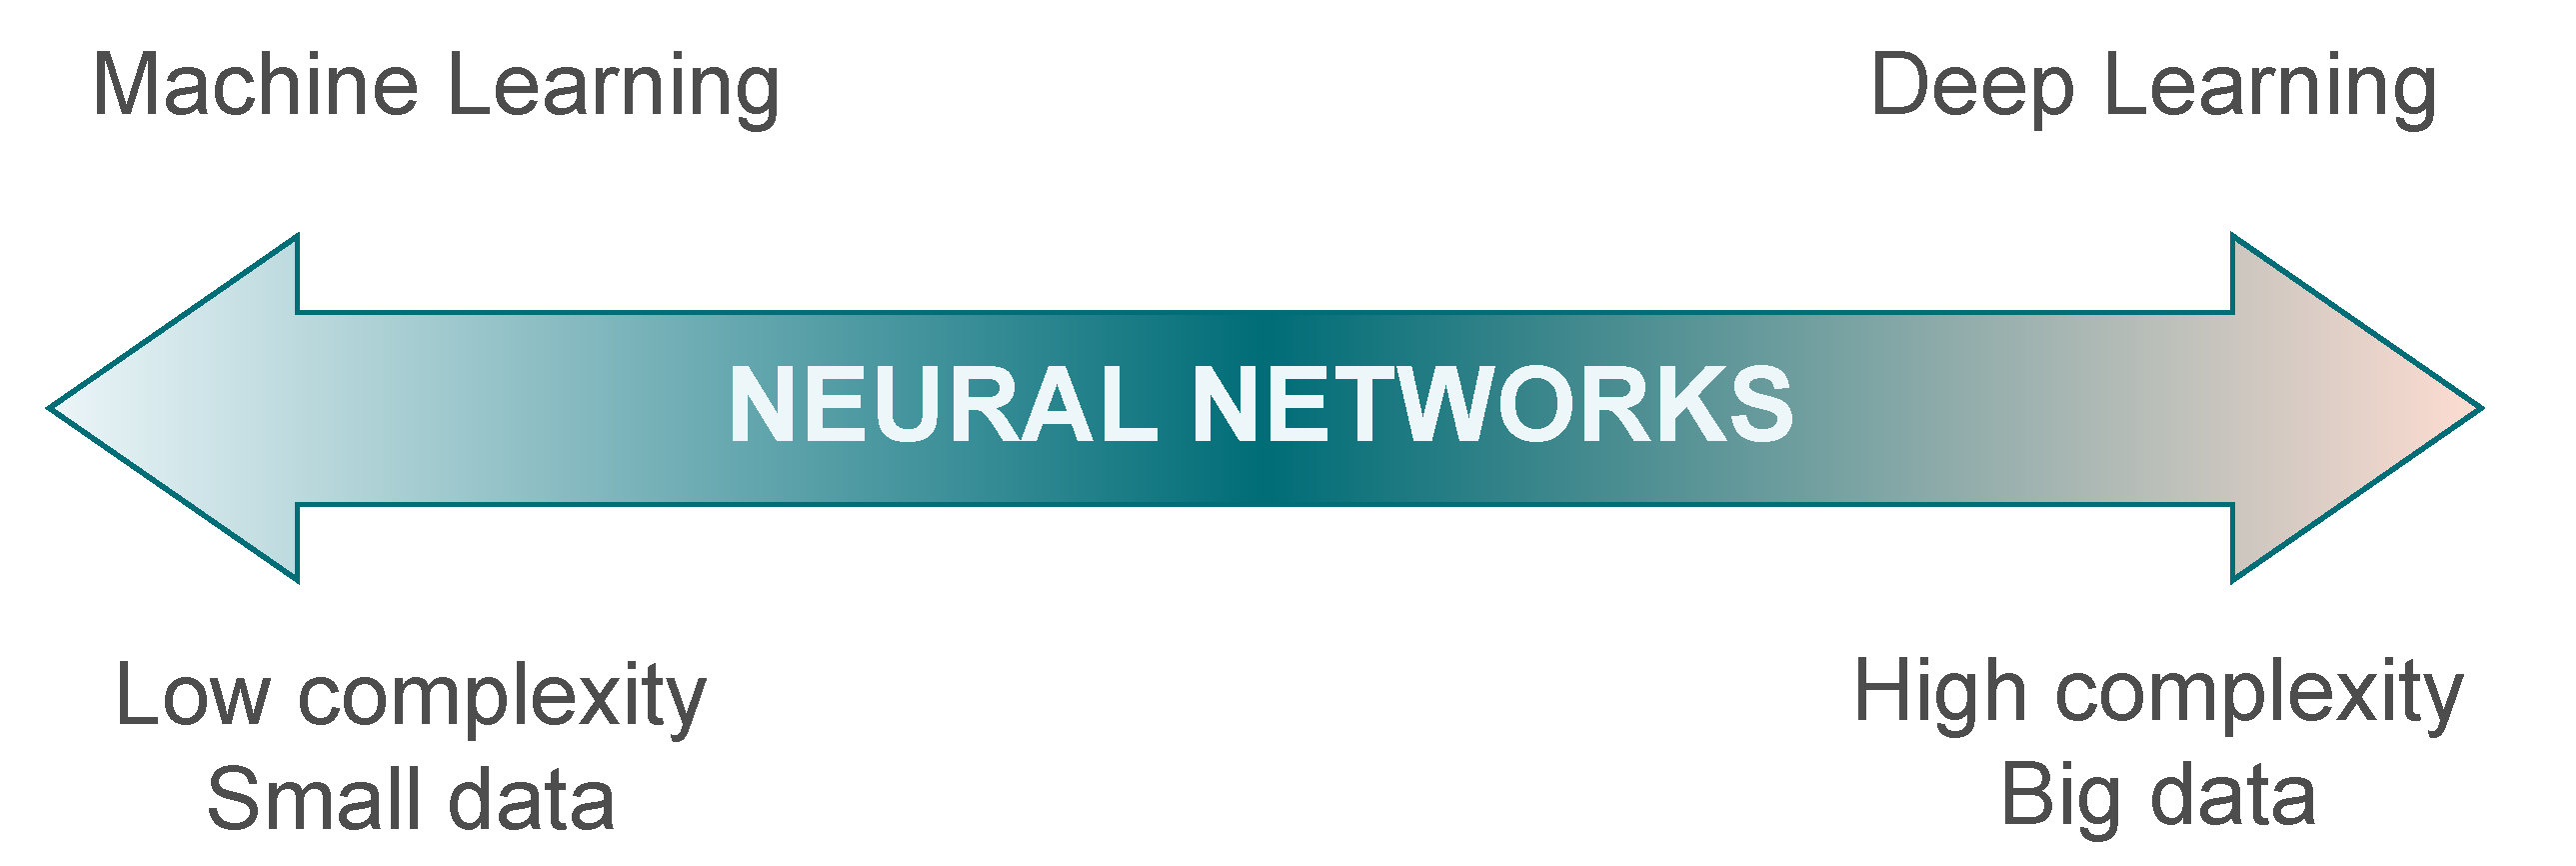
\includegraphics[width=0.8\linewidth]{NNvsMLvsDL.pdf}
  \caption{\alert{Neural networks} are a class of models that can be designed for different levels of complexity, from machine learning to deep learning problems.}
\end{figure}
\end{frame}




































%
% ---------------------------------------------------
% Section 3
% ---------------------------------------------------
% \section[\scshape\bfseries Neural Network Applications]{\scshape\bfseries Neural Network Applications}
%
% ---------------------------------------------------
% New frame
% ---------------------------------------------------



% %
% % ---------------------------------------------------
% % Section 4
% % ---------------------------------------------------
% \section[\scshape\bfseries Taxonomy of Learning Approaches]{\scshape\bfseries Taxonomy of Learning Approaches}
% %
% % ---------------------------------------------------
% % New frame
% % ---------------------------------------------------
% \subsection{Learning Approaches}
% \begin{frame}[allowframebreaks]{Introduction to Learning Approaches}
% Machine learning approaches can be grouped into four big families: 

% \vspace{0.5cm}
% \begin{enumerate}\justifying
% 	\item \alert{Supervised learning} is an approach based on data learning.

% 	\vspace{0.5cm}
% 	\item \alert{Unsupervised learning} is an approach aiming at clustering data even if no example is available. \alert{Self-supervised learning} is an unsupervised approach that allows of implementing supervised learning tasks.
	
% 	\vspace{0.5cm}
% 	\item \alert{Semi-supervised learning} is based on the availability of some examples, which are not enough to learn the model completely.
	
% 	\vspace{0.5cm}
% 	\item In \alert{reinforcement learning}, the optimal learning process aims at maximizing a certain \alert{\textit{reward}} associated to each action.
% \end{enumerate}

% \framebreak

% \vspace{1cm}
% \begin{figure}
% 	\centering
% 	\includegraphics[width=0.85\textwidth, keepaspectratio]{MLtasks2022.pdf}
% 	\caption{Representation of a taxonomy of machine learning approaches and tasks.} %
% \end{figure}

% \framebreak

% \vspace{1cm}
% \begin{figure}
% 	\centering
% 	\includegraphics[width=0.75\textwidth, keepaspectratio]{MLtasks_data.pdf}
% 	\caption{Representation of a taxonomy of machine learning approaches according to the availability of labelled or unlabelled data.} %
% \end{figure}
% \end{frame}
% %
% % ---------------------------------------------------
% % New frame
% % ---------------------------------------------------
% \subsection{Supervised Learning}
% \begin{frame}[allowframebreaks]{Supervised learning}
% \alert{\textbf{Supervised learning}} (SL) approach is based on the learning by data examples.

% \vspace{0.7cm}
% The examples, also denoted as \textit{training data}, can be seen as the available previous \linebreak experience, and based on this, one builds a model to make predictions for the future.
	
% \vspace{0.7cm}
% The main tasks in supervised learning are \alert{\textit{classification}} and \alert{\textit{regression}}, which will be \linebreak extensively studied during the course.

% \vspace{0.7cm}
% In SL, or \textit{learning with a teacher}, the network is provided with a correct answer (the \alert{output}) for every input.

% \framebreak
% A concise description of the data is provided by the \alert{supervisor function} that produces the output, given an input.

% \vspace{0.7cm}
% The supervisor function can be defined as a target signal $\mathbf{y}_k$ containing the desired output for a fixed set of inputs $\mathbf{x}_k$.

% \vspace{0.7cm}
% For this purpose, we define as \textit{training set} a given a set of empirical data defined over \linebreak input/output  space  ${\cal T} \subset ({ X}  ,{Y})$,  formally defined as
%  %
% \begin{equation*}
% 	\left[  \mathbf{x}_k , \mathbf{y}_k  \right]_{k=1}^K \in {\cal T} \left(\subset { X}  ,{Y}\right), \quad \mathbf{x} \in {X}  \subset  \mathbb{R}^P, \quad \mathbf{y} \in {Y} \subset \mathbb{R}^Q
% \end{equation*}
% %
% where $X$, $Y$ are, respectively, the input and output vector spaces.

% \framebreak
% The \alert{goal} of the SL is to find a suitable function that maps any input to an output space, in which a certain task can be accomplished. 

% \vspace{0.4cm}
% This process is subject to the minimization of a certain error.

% \vspace{0.2cm}
% \begin{figure}
% 	\centering
% 	\includegraphics[width=0.6\textwidth, keepaspectratio]{suplearn2022.pdf}
% 	\caption{General scheme for supervised learning.} %
% \end{figure}
% \end{frame}
% %
% % ---------------------------------------------------
% % New frame
% % ---------------------------------------------------
% \subsection{Unsupervised Learning}
% \begin{frame}[allowframebreaks]{Unsupervised learning}
% \alert{\textbf{Unsupervised learning}} (UL) aims at recovering the clusters in which the available data can be grouped together without relying on the availability of any previous example.

% \vspace{0.7cm}
% In UL, or \textit{learning without a teacher}, a correct answer associated to each input in the training set is not required.
% %
% %\vspace{0.7cm}
% %Hence, a concise description of the data could be a set of \alert{\textit{clusters}} or a probability density stating how likely it is to observe a certain object in the future.

% \vspace{0.7cm}
% UL explores the underlying \alert{\textit{structure}} in the data, or correlations between patterns in the data, and organizes input into categories from these correlations. 
% %
% %\vspace{0.7cm}
% %If some structure exists in training data, it can take advantage of the redundancy and find a short description of data.

% \vspace{0.7cm}
% A general way to represent data is to specify a \alert{similarity} between any pairs of objects. If they share any structure, it should be possible to reproduce the data from the same prototype.


% \framebreak
% \begin{figure}
% 	\centering
% 	\includegraphics[width=0.6\textwidth, keepaspectratio]{unsuplearn2022.pdf}
% 	\caption{General scheme for unsupervised learning.} %
% \end{figure}

% \vspace{0.5cm}
% The main UL tasks are \alert{\textit{clustering}} and \alert{\textit{dimensionality reduction}}. Typical \alert{examples} include \textit{image and text segmentation} and \textit{novelty detection} in process control.
% \end{frame}
% % Inserire figura
% %
% % ---------------------------------------------------
% % New frame
% % ---------------------------------------------------
% \subsection{Semi-Supervised Learning}
% \begin{frame}{Semi-supervised learning}
% \alert{\textbf{Semi-supervised learning}} is a hybrid approach that combines supervised and \linebreak unsupervised learning.

% \vspace{0.7cm}
% Input data is a \alert{mixture} of labeled (i.e., \textit{known}) examples (usually small quantity) and \linebreak unlabeled examples (larger quantity).

% \vspace{0.7cm}
% SSL may also be referred to as either:
% \vspace{0.2cm}
% \begin{itemize}\justifying
% 	\item \alert{transductive learning}, whose goal is to infer the correct labels for the given unlabeled data, 
% 	\vspace{0.2cm}
% 	\item \alert{inductive learning}, whose goal is to infer the correct mapping from $X$ to $Y$.
% \end{itemize}
% \end{frame}
% %
% % ---------------------------------------------------
% % New frame
% % ---------------------------------------------------
% \subsection{Self-Supervised Learning}
% \begin{frame}{Self-supervised learning}
% \alert{\textbf{Self-supervised learning}} is not really a hybrid approach, like semi-supervised learning, but it can be considered as an \alert{\textit{unsupervised learning approach}} as no labels were given.

% \vspace{0.6cm}
% However, \alert{unlike unsupervised learning}, it does not aim at clustering high-level patterns.

% \vspace{0.6cm}
% Indeed, self-supervised learning attempts to still solve tasks in a similar way to supervised learning, but \alert{without any label} available.

% \vspace{0.6cm}
% This is possible by \alert{augmenting the input data} using transformed versions of them.

% \vspace{0.6cm}
% This enables to \alert{learn group of similar classes}, which make possible tasks that originally required fixed labels to learn, such as classification, without any ground truth provided.
% \end{frame}
% %
% % ---------------------------------------------------
% % New frame
% % ---------------------------------------------------
% \subsection{Reinforcement Learning}
% \begin{frame}[allowframebreaks]{Reinforcement learning}
% The term \alert{\textbf{reinforcement learning}} (RL) refers more to a philosophy for learning algorithms development, which finds inspiration from behaviorist psychology, rather than to a specific type of algorithm.

% \vspace{0.8cm}
% RL has its roots in \textit{control theory}. 

% \vspace{0.8cm}
% Indeed, the typical RL scenario involves a \alert{\textit{dynamic environment}} that results in state-action-reward triples as the data.

% \vspace{0.8cm}
% The learning algorithm is intended as an \alert{\textit{agent}} working in a certain \alert{\textit{environment}}, which can take actions within it.

% \framebreak
% %\vspace{0.2cm}
% \begin{figure}
% 	\centering
% 	\includegraphics[width=0.5\textwidth, keepaspectratio]{reinflearn.pdf}
% 	\caption{General scheme for reinforcement learning.} %
% \end{figure}

% %\vspace{-0.1cm}
% For every \alert{action}, which is \textit{randomly} performed, a certain \alert{reward} can be related.

% \vspace{0.3cm}
% \alert{Randomness} may be introduced either as noise in \textit{measurements} or Monte Carlo randomness in the \textit{search procedure}, or both.

% \framebreak
% The difference between \textit{RL} and \textit{SL} is that in RL no optimal action exists in a given state, but the learning algorithm must identify an action in order to \alert{\textit{maximize the expected reward}} over time.

% \vspace{0.4cm}
% Unlike SL, the learning algorithm in RL is not told which actions to take in a given situation.

% \vspace{0.4cm}
% Instead, the learner is assumed to gain information about the actions taken by some reward not necessarily arriving immediately after the action is taken.

% \vspace{0.4cm}
% The \alert{\textit{concise description of data}} is the strategy that maximizes the reward.

% \vspace{0.4cm}
% An example of RL problem is \alert{\textit{learning to play chess}}.

% \framebreak
% One of the biggest \textit{challenges} of an RL algorithm is to find a trade-off between \alert{exploration} and \alert{exploitation}:

% \begin{itemize}\justifying
% 	\item[$-$] To maximize the reward, a learning algorithm must choose actions that have found to be \alert{\textit{effective in the past}} in producing a reward. 

% 	\item[$-$] %On the other hand, 
% 	To discover those actions the learning algorithm has to choose actions that was \alert{\textit{not tried in the past}}, thus exploring the state space.
% \end{itemize}

% \vspace{0.5cm}
% There is \alert{\textit{no general solution}} to this dilemma, but neither of the two options can lead exclusively to an optimal strategy.

% \vspace{0.5cm}
% RL is studied and applied in many disciplines, such as \textit{game theory}, \textit{stochastic/heuristic \linebreak optimization algorithms} involving random search and optimization, among others.
% \end{frame}
% %
% % ---------------------------------------------------
% % New frame
% % ---------------------------------------------------
% \subsection{Main Learning Tasks}
% \begin{frame}{Main learning tasks}
% \begin{figure}
% 	\centering
% 	\includegraphics[width=0.9\textwidth, keepaspectratio]{MLSPtasks2022d.pdf}
% 	\vspace{-0.2cm}
% 	\caption{In this course, we focus on both supervised and unsupervised tasks. Each task has a variety of applications that can be found in the real world.} %
% \end{figure}
% %
% %\framebreak
% %In particular, we will mainly deal with \textit{supervised learning} tasks, i.e.:
% \end{frame}



%
% ---------------------------------------------------
% Next Lecture
% ---------------------------------------------------
\begin{frame}{Summary and Further Reading}
Neural networks are \alert{composable}, \alert{differentiable} models that process \alert{complex data} via interconnected layers.

\vspace{0.6cm}
They represent a \alert{key approach} within machine learning and are at the heart of modern deep learning.

\vspace{0.6cm}
For more \alert{in-depth study}, consider resources such as:
\vspace{0.1cm}
\begin{itemize}\justifying
    \item {\small{Simone Scardapane, ``\myhref{https://www.sscardapane.it/alice-book/}{Alice’s Adventures in a Differentiable Wonderland}", 2024.}}
    \item {\small{Simon J. D. Prince, ``\myhref{https://udlbook.github.io/udlbook/}{Understanding Deep Learning}'', MIT Press, 2023.}}
    \item {\small{Aston Zhang, Zachary C. Lipton, Mu Li, and Alexander J. Smola, ``\myhref{https://d2l.ai/}{Dive Into Deep Learning}'', 2023.}}
\end{itemize}
\end{frame}
%
% ---------------------------------------------------
% Next Lecture
% ---------------------------------------------------
\section[Next Lecture]{}
\phantomsection
\begin{frame}{Next lecture}
\begin{itemize}\justifying
	\item The mathematics of neural networks
	\vspace{0.1cm}
	\begin{itemize}\justifying
		\footnotesize{
		\item[$-$] The notions of linear algebra that can be considered \alert{most relevant to neural networks} will be \linebreak introduced.
		\vspace{0.1cm}
		\item[$-$] Basic operations will be shown to \alert{process and manipulate} structured data.
		}\normalsize
	\end{itemize}
\end{itemize}
\end{frame}
%
% ---------------------------------------------------
% References
% ---------------------------------------------------
%\phantomsection
%%\begin{frame}[t,allowframebreaks]{References}\justifying
%\begin{frame}[t]{References}\justifying
%\nocite{*}\justifying
%\bibliographystyle{ieeetran}
%\footnotesize%\small 
%\justifying
%\bibliography{NN00refs}\justifying
%\end{frame}
%
% ---------------------------------------------------
% Thank you Page
% ---------------------------------------------------
\phantomsection
\begin{frame}[plain,t]{}
\vspace{-0.2cm}
\begin{beamercolorbox}[sep=1em,wd=\paperwidth,ht=2cm,dp=0.5cm,center]{postit} % One-line title
%\begin{beamercolorbox}[sep=0.5em,wd=\paperwidth,ht=2cm,dp=0.5cm,center]{postit} % Two-line title
	\usebeamerfont{title}{\MyBigTitle}\par
\end{beamercolorbox}
\vspace{0.7cm}
\begin{center}
	{\Large\scshape{\insertsubtitle}}\\
	
	\vspace{1.2cm}
	{\textcolor{redSap}{\textbf{\textsc{\insertauthor}}}}\\
	\vspace{0.4cm}
	\MyInstitute\\
\end{center}
\end{frame}
%
% ---------------------------------------------------
% End document
% ---------------------------------------------------
\end{document}
